\exo{ 0402 , tariel, 01/11/2017, 1-2, {}}[*, google]
Voici le plan d?une ville am�ricaine, G �tant la gare et H un h�tel :
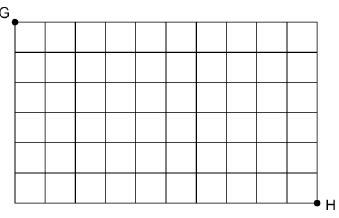
\includegraphics[width=0.25\textwidth]{chemin_court.png}

Chaque bloc est un carr� de 100 m sur 100 m. On cherche d'abord la longueur minimal en se d�pla�ant sur les segments:
\begin{itemize}
\item Comment faut-il se d�placer sur ce quadrillage
si on ne veut pas d�passer la longueur minimale ?
\item  Combien de d�placement pour la longueur minimale ?
\item  Combien de trajets diff�rents y a-t-il
pour aller de la gare � l'h�tel avec cette longueur minimale ?
\end{itemize}
\begin{correction}
\begin{itemize}
\item aller soit � droite soit vers le bas. Si on va gauche, le trajet se rallonge de deux car il faudra compenser en allant une fois � droite. Idem pour vers le haut 
\item 16 d�placements par exemple aller 10 fois � droite puis 6 fois vers le bas
\item On pose B = "vers le bas" et D = "vers la droite". Un exemple de chemin de G � H est le mot
BD...DBB...B o� B est �crit 6 fois et D est �crit 10 fois. Le nombre de chemins cherch� est clairement le
nombre d'anagrammes du mot pr�c�dent. Si on regarde la position du D dans un anagramme, on se ram�ne � un triage sans remise et sans ordre.
Donc le nombre de chemins est 6 parmi 16, soit $\begin{pmatrix}
16\\6
\end{pmatrix}$
\end{itemize}
\end{correction}

\finexo